\documentclass[12pt]{article}
\usepackage{fontspec}   %加這個就可以設定字體
\usepackage{xeCJK}       %讓中英文字體分開設置
\setmainfont{Times New Roman}
\setCJKmainfont{標楷體} %設定中文為系統上的字型,而英文不去更動,使用原TeX字型
\XeTeXlinebreaklocale "zh"             %這兩行一定要加,中文才能自動換行
\XeTeXlinebreakskip = 0pt plus 1pt     %這兩行一定要加,中文才能自動換行
\usepackage{amsmath, amsthm, amssymb} %引入數學符號的套件,例如實數R、定理Thm...
\usepackage{graphicx}                 %現在, 假設我們要插入 pic.png 這個圖檔, 使用
%\title{我是標題}
%\author{我是作者}
%\date{} %不要日期
\newcommand{\uA}       {\mbox{\boldmath$A$}}
\usepackage{textcomp}
\usepackage{array}
\usepackage{graphicx}
\usepackage{colortbl}
\usepackage{color,xcolor}
\usepackage{listings}
\usepackage{array,booktabs}   %這三個為表格使用的套件
\usepackage{textpos}
\usepackage{float}
\usepackage{listings}

\begin{document}
\begin{itemize}
\item[3.15]
(a)
\begin{verbatim}
znm=lm(crim~zn)
indusm = lm(crim~indus)
noxm = lm(crim~nox)
rmm = lm(crim~rm)
agem = lm(crim~age)
dism = lm(crim~dis)
radm = lm(crim~rad)
taxm = lm(crim~tax)
ptratiom = lm(crim~ptratio)
blackm = lm(crim~black)
lstatm = lm(crim~lstat)
medvm = lm(crim~medv)
\end{verbatim}
(c)\\
\centerline{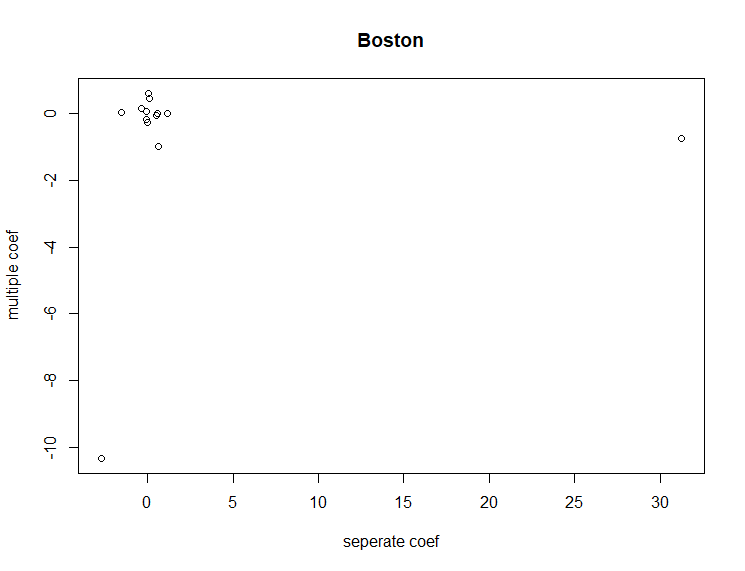
\includegraphics[width=0.8\linewidth]{boston}}\\
(d)
\begin{verbatim}
> bla=lm(crim~black+I(black^2)+I(black^3))
> summary(bla)

Call:
lm(formula = crim ~ black + I(black^2) + I(black^3))

Residuals:
    Min      1Q  Median      3Q     Max
-13.096  -2.343  -2.128  -1.439  86.790

Coefficients:
              Estimate Std. Error t value Pr(>|t|)
(Intercept)  1.826e+01  2.305e+00   7.924  1.5e-14 ***
black       -8.356e-02  5.633e-02  -1.483    0.139
I(black^2)   2.137e-04  2.984e-04   0.716    0.474
I(black^3)  -2.652e-07  4.364e-07  -0.608    0.544
---
Signif. codes:  0 ‘***’ 0.001 ‘**’ 0.01 ‘*’ 0.05 ‘.’ 0.1 ‘ ’ 1

Residual standard error: 7.955 on 502 degrees of freedom
Multiple R-squared:  0.1498,	Adjusted R-squared:  0.1448
F-statistic: 29.49 on 3 and 502 DF,  p-value: < 2.2e-16
\end{verbatim}
Through coding, we discover that there exists evidence of the non-linear association between all of the predictors and the response except for black.
\item[4.1]
$$P(X)=\frac{e^{\beta_{0}+\beta_{1}X}}{1+e^{\beta_{0}+\beta_{1}X}}$$
$$\frac{P(X)}{1-P(X)}=\frac{\frac{e^{\beta_{0}+\beta_{1}X}}{1+e^{\beta_{0}+\beta_{1}X}}}{\frac{1}{1+e^{\beta_{0}+\beta_{1}X}}}=e^{\beta_{0}+\beta_{1}X}$$
\item[4.2]
$$P_{k}(x)=\frac{\pi_{k}\frac{1}{\sqrt{2\pi}\sigma}\exp\{-{\frac{(x-\mu_{k})^2}{2\sigma^2}}\}}{\sum_{i=1}^{K}\pi_{i}\frac{1}{\sqrt{2\pi}\sigma}\exp\{-{\frac{(x-\mu_{i})^2}{2\sigma^2}}\}}$$
$$\delta_{k}(x)=x\frac{\mu_{k}}{\sigma^2}-\frac{\mu_{k}^2}{2\sigma^2}+\log(\pi_{k})$$
Let\ $\delta_{k}(x)>\delta_{i}(x)$, $\forall i\neq k$\\[3ex]
Since exponential function is monotone increasing:
$$
\exp(\delta_{k}(x))>\exp(\delta_{i}(x))\\
\Rightarrow\pi_{k}\exp(\frac{\mu_{k}}{\sigma^2}-\frac{\mu_{k}^2}{2\sigma^2})>\pi_{i}\exp(\frac{\mu_{i}}{\sigma^2}-\frac{\mu_{i}^2}{2\sigma^2})
$$
thus we prove that maximizing\ $\delta_{k}(x)$ is equivalent to maximizing\ $p_{k}(x)$.
\item[4.3]
$$P_{k}(x)=\frac{\pi_{k}\frac{1}{\sqrt{2\pi}\sigma_{k}}\exp\{-{\frac{(x-\mu_{k})^2}{2\sigma_{k}^2}}\}}{\sum_{i=1}^{K}\pi_{i}\frac{1}{\sqrt{2\pi}\sigma_{i}}\exp\{-{\frac{(x-\mu_{i})^2}{2\sigma_{i}^2}}\}}$$
Since we assume that the\ $\sigma^2$ of each class is not same, so we can't remove the\ $\sigma^2$.
\begin{align*}
\delta_{k}(x)
&=\log(P_{k}(x))+\log(\sum_{i=1}^{K}\pi_{i}\frac{1}{\sqrt{2\pi}\sigma_{i}}\exp\{-{\frac{(x-\mu_{i})^2}{2\sigma_{i}^2}}\})\\
&=\log(\pi_{k})-\log(\sqrt{2\pi}\sigma_{k})-\frac{(x-\mu_{k})^2}{2\sigma_{k}^2}
\end{align*}
It is not linear, and we can see that it is quadratic.
\end{itemize}
\end{document} 